\chapter{SYSTEM ANALYSIS}

It deals with the analyzing of the entire system i.e.  the  different  entities  and  the interaction between  those entities and also  the different  functionalities of  the system.  It consists of performance analysis,  It also consists  of  the  specification  of  different  types  of  requirements  like  software  requirements, communication requirements, database requirements etc.   


\section{System Model}
\hspace{1cm}The software system has been designed into two levels. At the first level the focus is on deciding which modules are needed for the system, the specification of these modules and how the modules should be interconnected.  This is called as system design or top level design. In the second level, the internal design of the modules or how the specifications of the module can be satisfied is decided. This design level is often called detailed design or logic design.  \cite{DBLP:journals/ivc/KadyrovP03}.\\
\paragraph\ When the user clicks on the application icon, this game is launched in the windows phone.
When the game is launched the first page or the menu page of the game is displayed.
The menu page consists of two buttons, PLAY and EXIT.
At the click of the play button, the introduction of the game is started. Here, the characters of the game is introduced, and tells the user the storyline of the game.
After the introduction of the game different levels of the game is started. When the user loses all the attempts or if the time-out occurs, the user is displayed with a “game over”. Where the game control is navigated to the Menu page. 
Throughout the game the images for the game are accessed from the database, and the audio player agent is linked to the game to play the audio at the background.
 \cite{DBLP:journals/ivc/KadyrovP03}.\\
\begin{figure}[htbp]
	\centering
	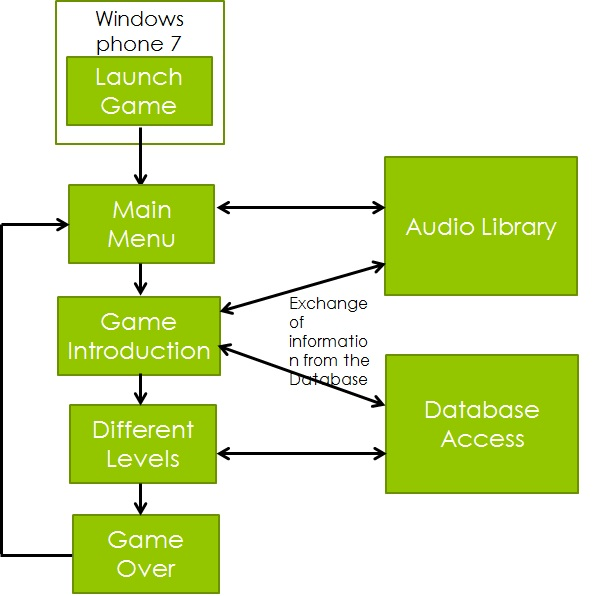
\includegraphics[width=10cm,height=6cm]{system.jpg}
	\caption{System Model}
\end{figure}

\section{Functional Requirements}
\hspace{1cm}Include all the functional requirements mentioned in the presentation slides with respect to your application. (not individual functional requirements are expected)
\\ \hspace{0.5cm}1.At the start of the application, the main menu page shall be displayed.The main menu shall consist of 2 buttons, PLAY and EXIT.
\\2. At the click of PLAY button, the user shall be given an option to enable or disable the sound of the application.
\\3. If the user enables sound then background audio shall be played using background audio player agent. 
\\4.	After enabling/disabling of the sound the application shall be navigated to the next page.
\\5.	The next page of the application shall introduce the story to the user.
\\6.	In this application .gif shall be used to enable the animation and the motion of the images. 
\\7.	During gameplay different set and type of questions shall be displayed on screen and answers shall be validated before proceeding to next step.
\\8.	Different set and type of questions and all the solutions shall be stored in an isolated file storage medium i.e. mobile’s flash memory. 
\\9.	At a different level of game suitable type of question must be fetched from file and displayed on screen.
\cite{DBLP:journals/ivc/KadyrovP03}.\\

\section{External Interface Requirements}
\hspace{1cm}There are many additional hardware and software which are required
for the development of any of the software application; they also constitute
a major part in the application. This section provides the overview of the
external interfaces used for the development of the Mystery Doors.
 \cite{DBLP:journals/ivc/KadyrovP03}.\\


\subsection{Hardware Interfaces}
\begin{itemize}
\item \textbf {}Windows mobile phone 
\item \textbf {}128Mb RAM
\item \textbf {}Minimum storage space on hard disk is 15Mb. 
\end{itemize}

\subsection{Software Interfaces}
\begin{itemize}
\item \textbf {}Visual Studio Express for Windows Phone.
\item \textbf {}Windows phone emulator.
\end{itemize}

\section{User Requirements}
\begin{itemize}
\item \textbf {Home Screen}: The  first  screen  to be displayed which allows user  to enter the user to start the game. 
\item \textbf {GUI}: When  the  user  chooses  some  other option,  then  the  information  pertaining  to that choice will be displayed on to the screen.
\item \textbf {Notifications}: When  the user loses, then the necessary message like “game over” will be displayed. 
\end{itemize}
\section{Performance Requirements}
\hspace{1cm}
Performance requirements coincide with the Windows platform limitations. 
\begin{itemize}
	\item \textbf {Memory}- Our app requires maximum of 15 Mb memory.
	\item \textbf {Response time}- This app’s response time is 0.5s.
	\item \textbf {Speed}- Depends on the mobile’s main memory.
	\item \textbf {Portability}- Meets out all the requirements of the customer.
	\item \textbf {Performance}- The performance is better if the user downloads the app properly.

\end{itemize}


